\section{Assinatura baseada em Scene Frames}

% Traduzir scene frame?

Outra abordagem, proposta por \citeauthormao2015sceneframe}, é baseada na assinatura de \textit{scene frames}, ou quadros de cena. O algoritmo fundamenta-se na ideia de que as chances de existirem cinco quadros de cena seguidos é extremamente baixa. De acordo com os autores, um quadro de cena pode ser representado tanto por quadros de referência (chamados \textit{intraframes}), quanto pelos quadros que são codificados pelo mesmo (\textit{interframes}), contanto que siga duas características: o quadro deve ser uma imagem no formato espacial; e os mesmos objetos, além de um \textit{background} altamente similar, devem pertencem a uma mesma cena.

\subsection{A extração de assinatura}

Primeiramente, todo quadro é pré-processado, seguindo uma série de passos que serão descritos a seguir:

\begin{enumerate}
	\item O componente de luminância é obtido
   	\item O quadro é recortado, utilizando-se apenas sua área central
    \item O quadro é redimensionado para o tamanho de $3/4$QCIF, ou seja, $(108\times132)$
\end{enumerate}

Após o processamento inicial, o quadro é então dividido em $144$ pedaços menores, de tamanho $(9\times11)$, cuja média de intensidade irá compor parte da assinatura deste quadro. Além dos $144$ valores, o descritor é composto também por $576$ elementos diferenciais, totalizando $720$ valores. Para obter esses elementos, cada fragmento é dividido em oito elementos menores, como mostra a Figura \ref{fig:divsceneframe}, e então é realizada a subtração de $a - b$, $c - d$, $e - f$ e $g - h$.

\begin{figure}[h]
	\centering
    \label{fig:divsceneframe}
	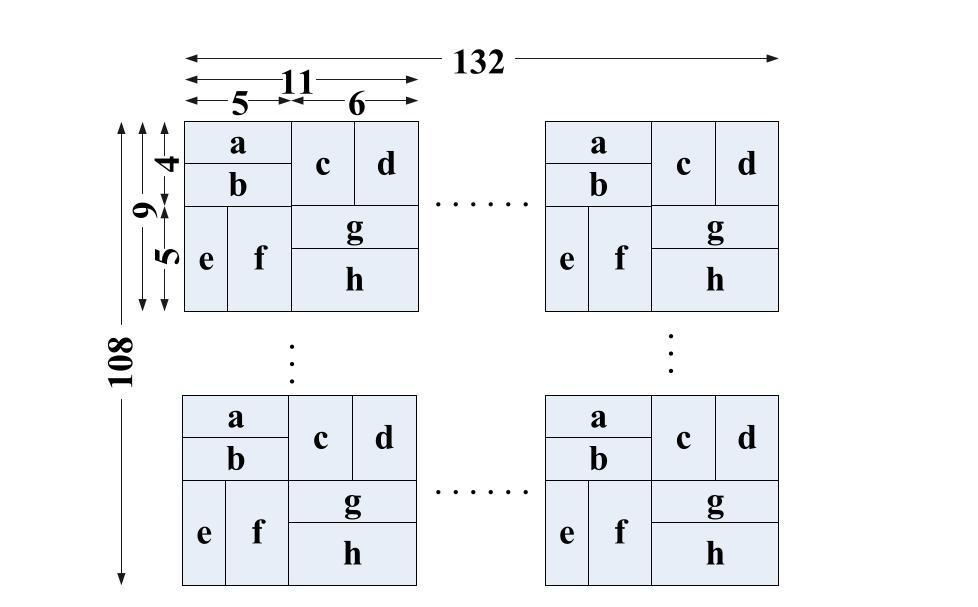
\includegraphics[width=\textwidth]{dados/figuras/divisaosceneframe.jpg}
    \caption{Divisão da imagem para cálculo dos elementos diferenciais. Referência: \citeauthormao2015sceneframe}}
\end{figure}

\subsection{Diminuição do espaço de memória utilizado}

O artigo também propõe uma alternativa para diminuir o espaço de memória utilizado para armazenar as assinaturas, visto que o banco de dados dos vídeos pode ser grande. Para isso, é proposta uma técnica chamada qualificação quaternária, na qual os valores são classificados de acordo com um \textit{threshold}.



